%%----------------------------------------------------------------------
\section{Overview}
\label{s:Overview}
%% - - - - - - - - - - - - - - - - - - - - - - - - - - - - - - - - - - -

Project CASSIA (Comprehensive Architecture of Social Simulation for
Inclusive Analysis) aims to develop a framework to administer 
execution of large-scale multiagent simulations exhaustively to analyze
socially interactive systems. The framework will realize engineering
environment to design and synthesize social systems like traffics,
economy and politics.

The purpose of multi-agent social simulation is to provide
tools to design social systems.
It is impossible or quite difficult to carry out experiments
of social phenomena in the real world 
by the similar way as experiments in physics or chemistry.
Therefore, computational social simulations are indispensable means
for social science.

Fortunately,
progress of computational power has a potential to realize wider applications of
computer simulation not only in physical phenomena but also in social 
problems.
High performance computing (HPC) has been enabling several simulation researches
on large-scale weather, molecular dynamics, structures and architectures, and
disasters.
In addition to these physical phenomena,
recently,
social phenomena like economics, traffics, or information flow on
networks
attract many attentions as applications of HPC.

In order to make such social simulations on HPC
available for wide-range users,
the CASSIA framework consists of:
\begin{itemize}
  \item
    MASS Planning Module: a manager module conducts effective
    execution plans of simulations among massive possible conditions
    according to available computer resources.
  \item
    MASS Parallel Middleware: an execution middleware provides
    functionality to realize distributed multi-agent simulation on
    many-core computers.
\end{itemize}

%%++++++++++++++++++++++++++++++++++++++++++++++++++++++++++++++++++++++
\begin{figure}
  \centering
  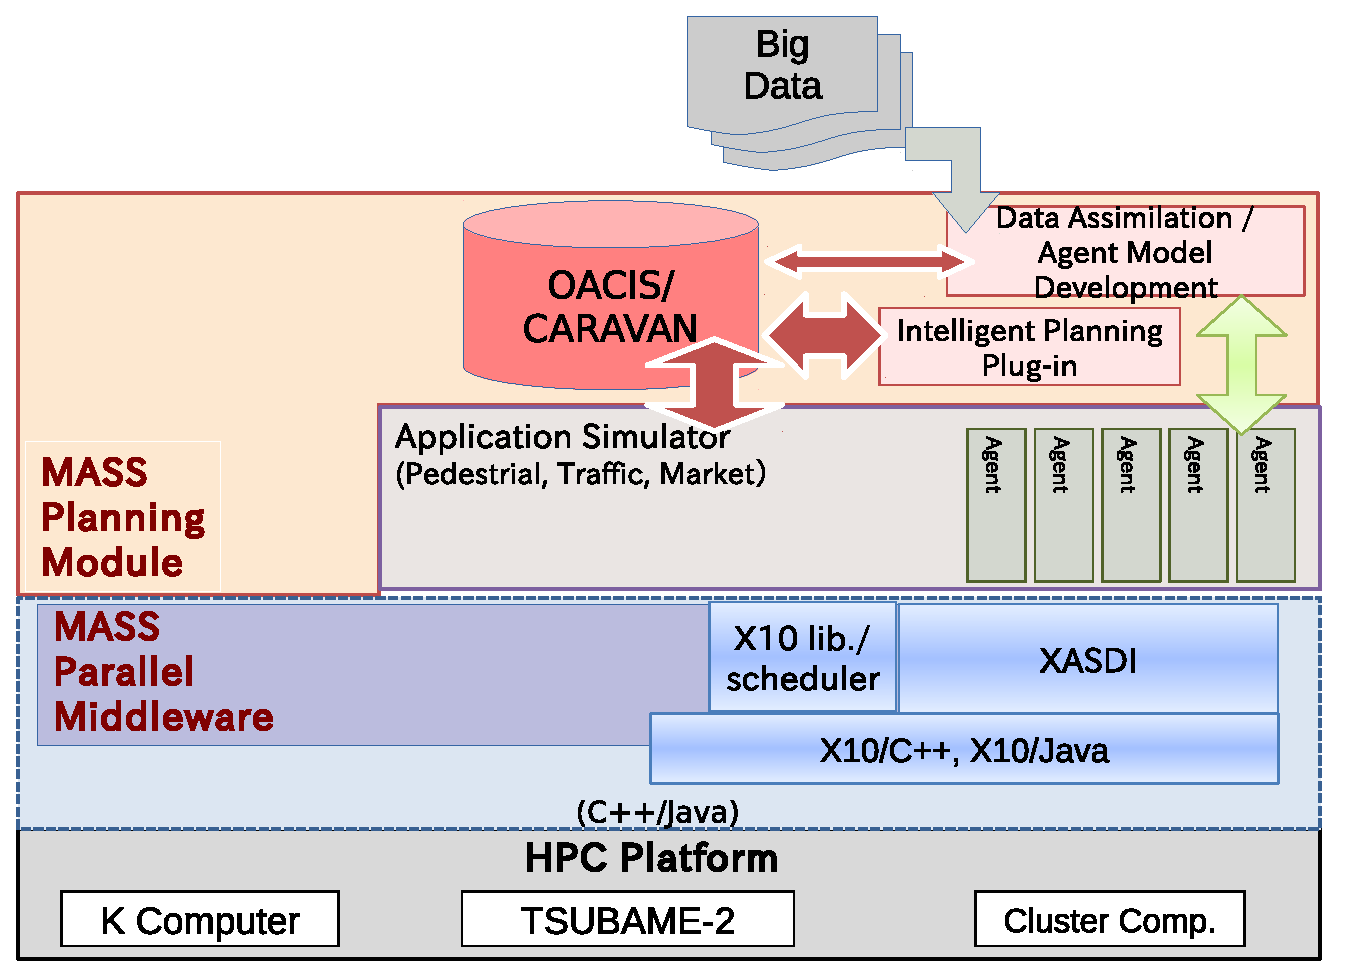
\includegraphics[width=.8\linewidth]{Figs.noda/figure-01.framework.eps}
  \caption{Cassia Framework}
  \label{fig:Figs.noda/figure-01.framework.eps}
\end{figure}
%%++++++++++++++++++++++++++++++++++++++++++++++++++++++++++++++++++++++

